\documentclass[conference]{sty/IEEEtran}
\usepackage{times}
\usepackage{wrapfig}
\usepackage{tweaklist}
\usepackage{xspace}
\usepackage{graphicx}
\usepackage{tabularx}
\usepackage{amsmath}
\usepackage{amssymb}
\usepackage{url}
\usepackage{bm}
\usepackage{color}
\usepackage{colortbl}
\usepackage{subfig}

\def\cH{\mathcal{H}}
\def\cL{\mathcal{L}}
\def\cP{\mathcal{P}}
\def\cO{\mathcal{O}}
\def\mP{{\mathsf P}}
\def\mh{{\mathsf h}}
\def\mo{{\mathsf o}}
\def\mv{{\mathsf v}}
\def\mn{{\mathsf n}}
\def\vcb{{\boldsymbol{c}}}
\def\vpb{{\boldsymbol{p}}}
\def\vqb{{\boldsymbol{q}}}
\def\vnb{{\boldsymbol{n}}}
\def\vlb{{\boldsymbol{l}}}
\def\mr{{\mathsf r}}


% numbers option provides compact numerical references in the text.
\usepackage[numbers]{natbib}
\usepackage{multicol}
\usepackage[bookmarks=true]{hyperref}

% \pdfinfo{
%    /Author (Homer Simpson)
%    /Title  (Robots: Our new overlords)
%    /CreationDate (D:20101201120000)
%    /Subject (Robots)
%    /Keywords (Robots;Overlords)
% }

\begin{document}

% paper title
%\title{Classification of Objects of Daily Use Using Combined Color CHLAC and Global Radius-based Surface Descriptors}
%\title{Multidimensional Descriptor for Classification of Objects of Daily Use}
\title{Voxelized Shape and Color Histograms for RGB-D}

% You will get a Paper-ID when submitting a pdf file to the conference system
\author{Paper-ID [110]}

% \author{\authorblockN{Asako Kanezaki, Tatsuya Harada}
% \authorblockA{
% Graduate School of Information \\ Science and Technology,\\
% University of Tokyo \\ %7-3-1 Hongo Bunkyo-ku, Tokyo Japan \\
% Email: \{kanezaki, harada\}@isi.imi.i.u-tokyo.ac.jp}
% \and
% \authorblockN{Dejan Pangercic, Zoltan-Csaba Marton, Michael Beetz}
% \authorblockA{
% Intelligent Autonomous Systems Group,\\ TU Munich \\
% Email: \{pangercic, marton, beetz\}@cs.tum.edu}}

\newcommand{\todo}[1]{\textbf{\textcolor{red}{TODO: #1}}}
\maketitle

\begin{abstract}
Object detection plays an important role in autonomous manipulation,
but it faces many challanges. Several objects have similar color
or shape, so a descriptor is needed that takes both into account
efficienlty and with high discriminating power. In this paper we
present an approach to efficiently capture these two dimensions
into a single feature
% % % The greatest bottleneck momentarily in the area of mobile manipulation is robust perception.
% % % In this paper we contribute to the solving of this problem of efficiency and accuracy
% % % by proposing a novel feature called Voxelized Shape and Color Histograms 
% % % (VOSCH)
that is capable of capturing both the geometric and visual appearance
properties of common objects of daily use. We showcase the
feature's applicability for the purpose of classification of objects in cluttered scenes with occlusions,
and evaluate two classification approaches.
For the experiments we make use of a new RGB-D device Kinect, and achieve recognition
rates higher than \emph{85\%} for a set of 63 objects.
\end{abstract}

\IEEEpeerreviewmaketitle

\section{Introduction}
One of the great challenges in autonomous mobile robot manipulation is scaling
technology to realistic tasks, in real-world environments under realistic
conditions. This means that an autonomous household robot must act on many
different objects of daily use, handle them in typical situations such as
opening a fridge to get the milk or when performing challenging everyday tasks
such as setting the table or preparing a meal.

%\todo{Provide the definition of descriptor vs detector vs feature}\\
Descriptor-based object recognition has proved over last years to be very successful.
SIFT~\cite{lowe04distinctive}, SURF~\cite{surf} and others can
detect, localize and recognize many types of textured objects efficiently, reliably
and under varying lighting conditions. Likewise descriptors have been developed 
for perceiving objects based on their shapes (e.g. circles, cylinders, spheres and hybrid variants).
Normal Aligned Radial Features (NARF)\cite{steder10irosws} for range images, 
and several versions of Point Feature  Histograms (PFH, FPFH)~\cite{Rusu09ICRA} and 
Viewpoint Feature Histograms (VFH)~\cite{vfh} for unordered fully-3D point clouds are just 
to name a few. While these descriptors were successful too, they are still limited because they
typically work only in restricted feature spaces. So, in order to have a perception system
based on SIFT features, one needs to restrict the search space to objects that are detected by
texture ane if we apply 3D feature the objects must be distinctive with respect to their shapes. 
If we want to install a perception system for autonomous robots we need to aim 
at one that can perceive all objects, that is textured, texture-less, different shapes, etc.

While it seems feasible that one can simply develop perception routines by combining
various descriptors~\cite{stueckler10combining, GRSD10Humanoids}, but a promising idea 
is to develop descriptors that work in multiple feature spaces. The reason for this is 
that objects might be easily discriminated in a combined feature space whereas it is impossible 
to discriminate them in individual spaces as depicted in Figure~\ref{fig:grsd_cchlac}.
Our approach is thus to be seen as an alternative to the bag-of-experts type
of approaches~\cite{Varma07learningthe}.

In this paper we report on our work on the two variations of a novel descriptor
which builds off the idea of the previously 
published Global Radius-based Surface Descriptor (GRSD~\cite{GRSD10Humanoids}) and the
Color Cubic Higher-order Local Auto-Correlation descriptor (ColorCHLAC~\cite{kanezaki2010tvc}).
We termed it (Concatenated) Voxelized Shape and Color Histograms -- (Con)VOSCH.

\begin{figure}[htb!]
  \begin{center}
    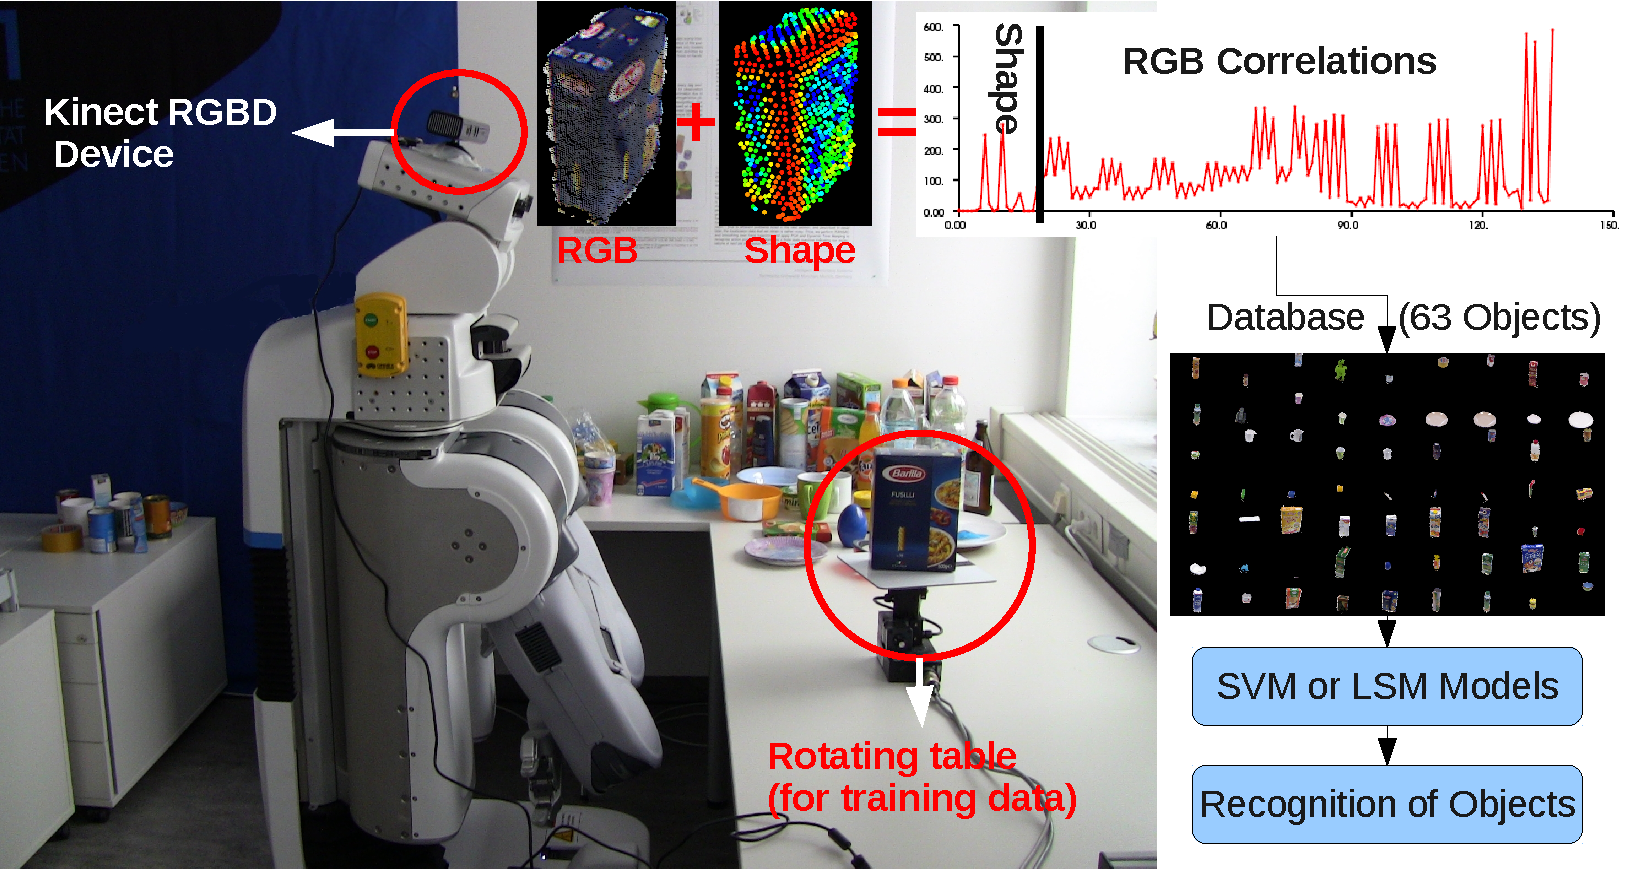
\includegraphics[width=.99\columnwidth]{figures/firstpage/firstpage.pdf}
    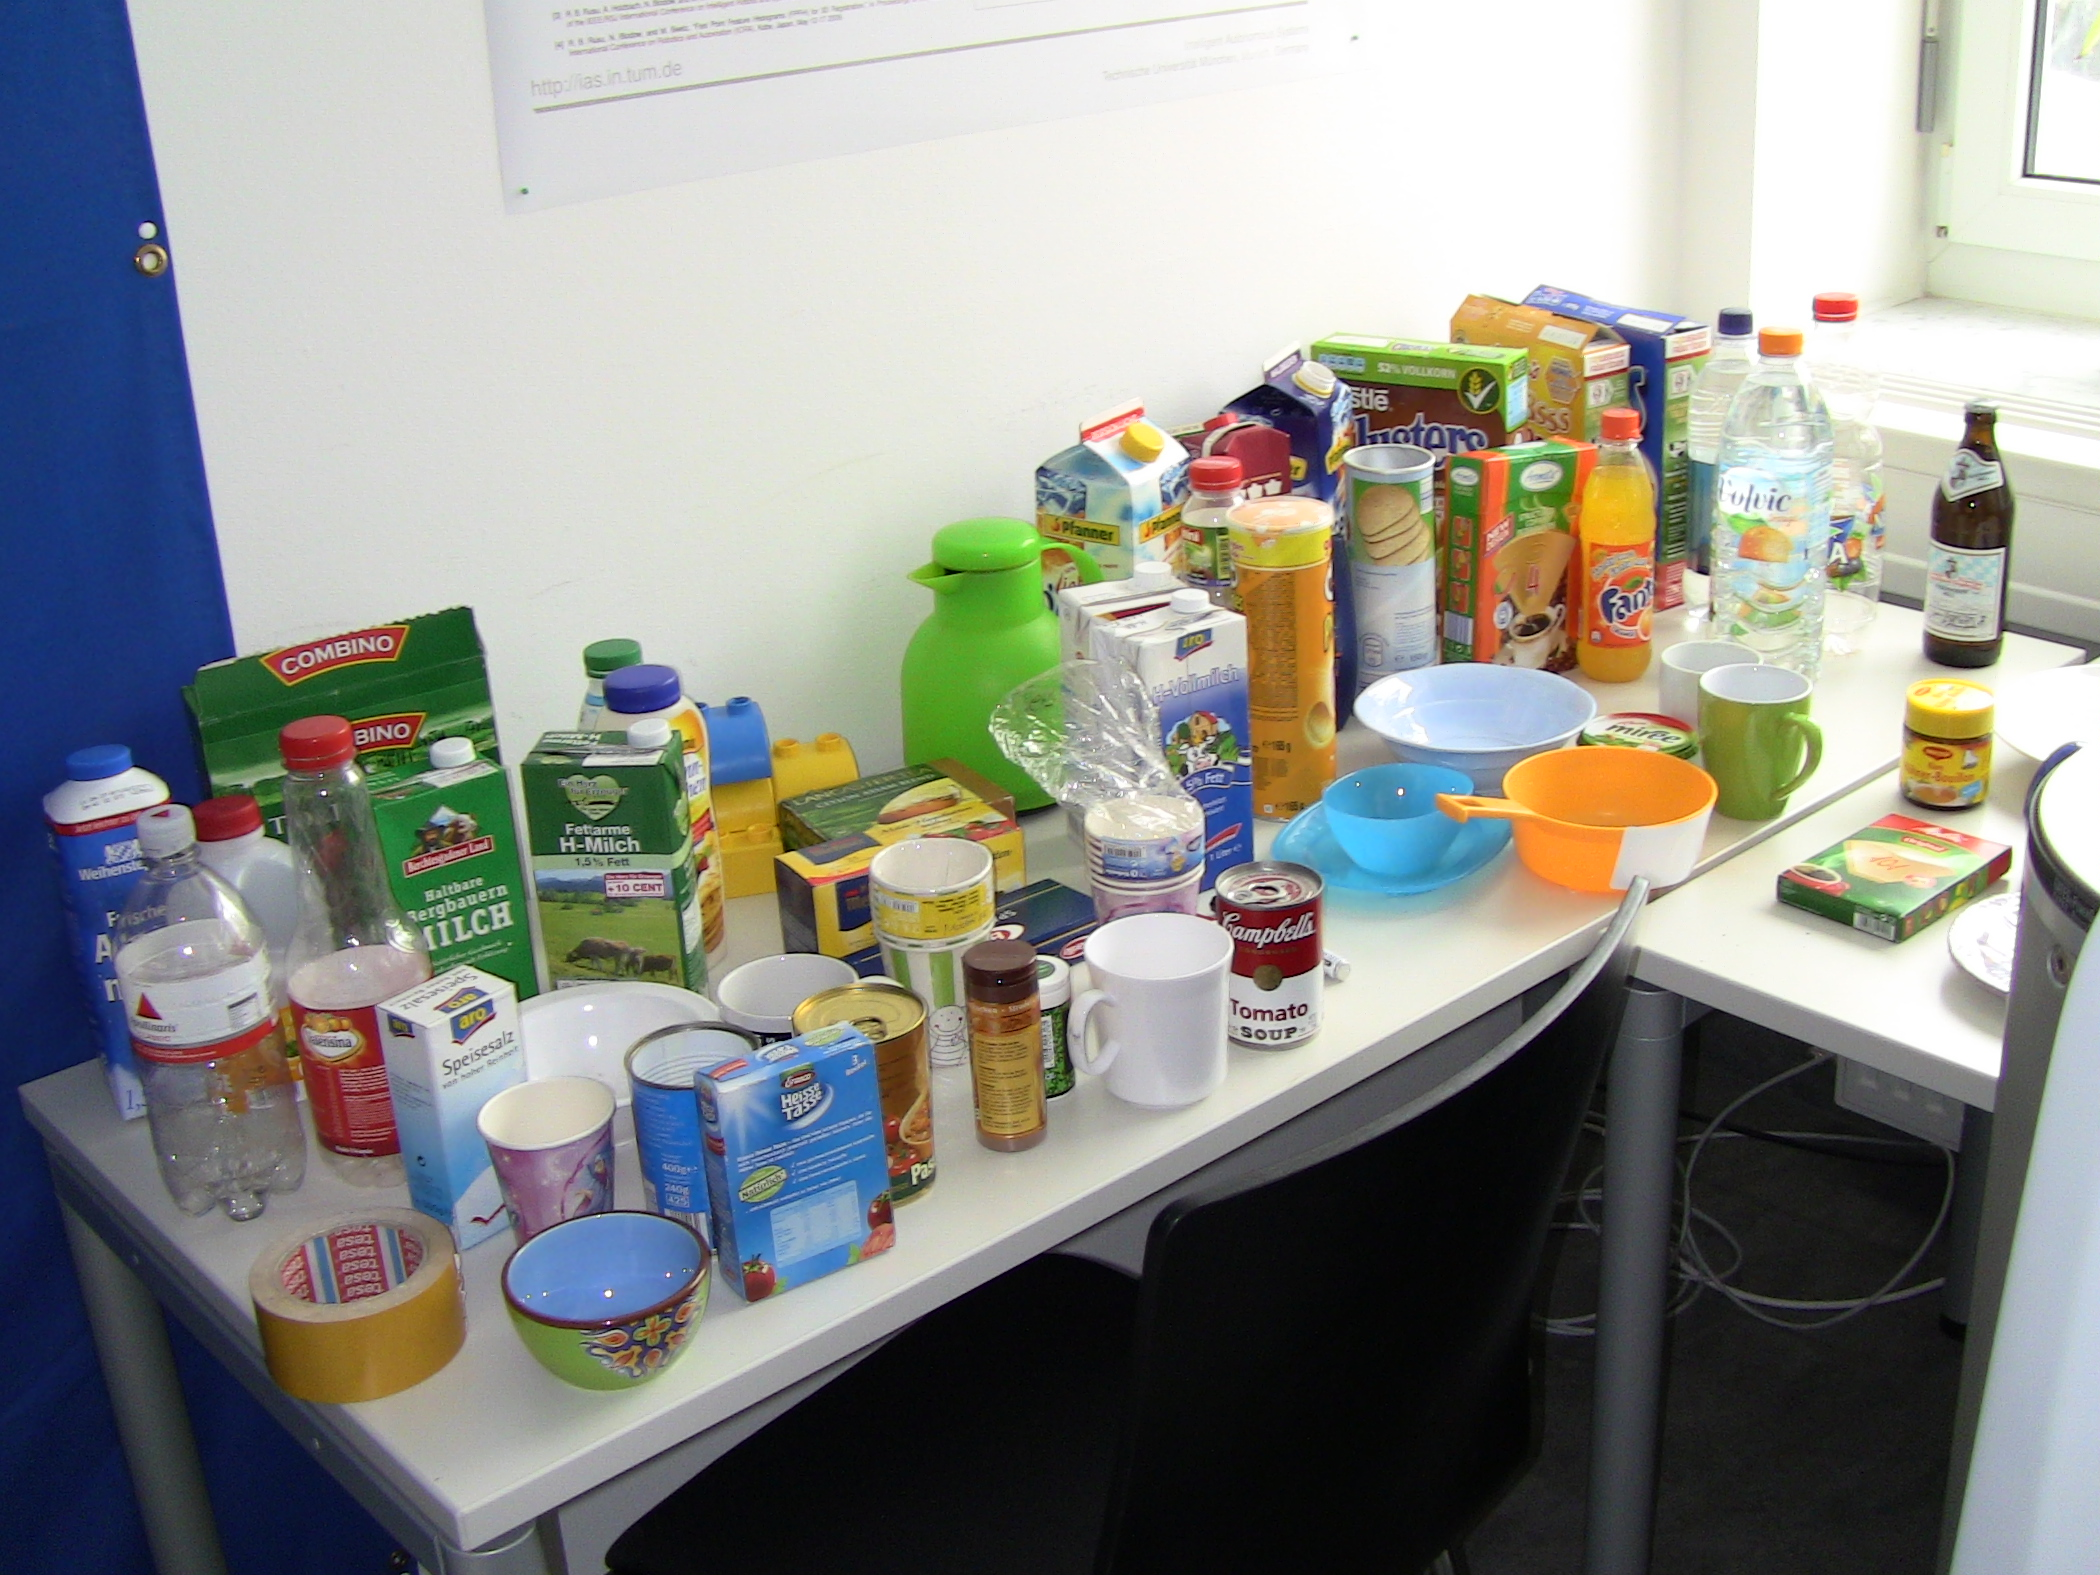
\includegraphics[width=.99\columnwidth]{figures/objects/objects.jpg}
    \caption{Top: Autonomous service robot equipped with a Kinect sensor
    acquiring training data of the objects shown in the bottom image. For 
  every view of the object VOSCH or ConVOSCH descriptor was estimated and a database
of 63 objects was generated. Object detection pipeline with Support Vector
Machine or Linear Subspace Method classifiers was then used to detect objects
in natural scenes.}
    \label{fig:robot}
  \end{center}
\end{figure}

% \subsection{What}
% In this paper, we address the problem of localization and recognition of
% objects of daily use in households. To this effect, we employ a multidimensional
% feature descriptor that captures both the geometrical and visual appearance
% properties of the objects.

The strength of the descriptor lies in its ability to consider geometric and
visual features in a unified manner to facilitate object classification. The two
underlying features (GRSD, ColorCHLAC) have been carefully selected because of 
their similar structures and the way they are computed from voxelized 3D data. 
While ConVOSCH is a mere concatenation of GRSD and ColorCHLAC histograms, we 
developed VOSCH such that allows for its computation in a single step because 
of the modified underlying algorithmic properties for GRSD and ColorCHLAC. 
Both features count relations between neighboring voxels, capturing geometric 
surface type and texture transitions at the same time.

Further contributions of work presented herein include the ability to deal with
cluttered scenes while eliminating the requirement for region of interest
selection (e.g. horizontal supporting structures) and spatially separable object
clusters. This has been achieved by ensuring that the descriptor is additive, and using a
moving-bounding-box-based approach together with a sub-space-matching-based classification scheme (Section
\ref{sec:recognition}). The resulting approach performs at 2 frames per second
while taking into account an object database of 63 different objects
(see Figure~\ref{fig:robot}).


% \subsection{Why}
% In the past, strong features have been proposed in perception for personal robots,
% both working on 2D and 3D data. Prominent examples include
% SIFT~\cite{lowe04distinctive} and SURF~\cite{surf} for camera images, Normal Aligned Radial
% Features (NARF)\cite{steder10irosws} for range images, and several versions of Point Feature
% Histograms (PFH, FPFH)~\cite{Rusu09ICRA} and Viewpoint Feature Histograms
% (VFH)~\cite{vfh} for unordered fully-3D point clouds.
% \todo{Nico proof-read till here}


% Yet it seems that there is none that can capture
% all important and obvious properties (such as geometry and color are)
Lastly, our descriptor can be out-of-the box applied on the data coming from the 
new sensing technologies such as Kinect device and lays the foundation stone for a
multitude of applications such as later discussed detection of a priori learned object models
(Section~\ref{sec:recognition}).
% % % VOSCH also enables equipping of service robots 
% % % (such as the robot shown in top part of Figure~\ref{fig:robot}) with the 
% % % capabilities to acquire additional object models which furthermore opens ways 
% % % for manipulation tasks in realistic environments under realistic conditions.

\begin{figure}[htb!]
  \begin{center}
    \includegraphics[width=.48\columnwidth]{figures/colorCHLAC/artificial/purple.png}
    \includegraphics[width=.48\columnwidth]{figures/colorCHLAC/artificial/torus.png}
    \caption{Examples of \todo{scaled} VOSCH histograms.
Left: different categories of objects (top-down: cone, cube, cylinder, plane, sphere, torus, dice) 
result in having different first 20 bins of the respective histogram.
Right: different colors of the same category of an object torus have different 117 right-most bins of the histogram}
    \label{fig:grsd_cchlac}
  \end{center}
\end{figure}

The remainder of the paper is built as following. After the overview of the related
work in Section~\ref{sec:rl} we present a system overview in Section~\ref{sec:overview}
which is followed by Section~\ref{sec:features} that elaborates on the construction of the
ConVOSCH and VOSCH descriptor variants. In Section~\ref{sec:classification} we present the usage of this descriptor
for the classification of objects using two classification methods which we
then test and present in Section~\ref{sec:results}. In Section~\ref{sec:conclusion}
we conclude and give an outlook on our future work.

\section{Related Work}
\label{sec:rl}
%\item Color CHLAC (Asako)~\cite{kanezaki2010icra}\cite{kanezaki2010tvc}
% \item textured-spin images~\cite{Johnson_spin_images}
% \item A sparse texture representation using local affine
% regions~\cite{Lazebnik05asparse}
% \item sift-keypoint
% \url{http://www.ros.org/doc/api/pcl/html/sift__keypoint_8h_source.html}
Expressiveness and efficiency of the descriptor are both crucially important for
a real-time object recognition system.  Though there is a trade-off between
these two abilities, it will improve both of them to select a
proper matching method which accounts for the characteristics of the
descriptor. In the recent decade a corpus of powerful 2D and 3D descriptors for
recognizing real objects have been developed, however, few of them take into
account the compatibility with the matching method used with them.

SIFT~\cite{lowe04distinctive} descriptor, one of the most well-known 2D
descriptors for object recognition, makes use of detected keypoints in
scenes and compares them with those of reference objects to identify the
objects currently observed. A combination of the visual appearance
descriptor and 2D shape is presented by Bosch et al. in~\cite{Bosch07shape}
where they use random forests to achieve around 80\% of classification 
accuracy. 

NARF~\cite{steder10irosws} descriptor detects salient points in range images of
real environments. Despite of its dominant
repeatability in point-to-point matching, there still remains difficulty in
cluster-to-cluster matching, which is necessary for identifying each cluster
candidate as object in the environment. This also causes high computational cost
especially when the target object database is large. In a 3D domain a recently 
developed VFH~\cite{vfh} descriptor was presented as an extension 
of~\cite{Rusu09ICRA}. The feature's discriminative power is boosted up
by inclusion of the viewpoint which on the other side also represents
the deficiency in that it becomes orientation variant. 

There are few approaches that use both geometry and color descriptors to
represent 3D shapes~\cite{park2006}, however properly balancing these two
different properties is difficult.  Caputo and Dorko~\cite{caputo2002} learned
respective kernels for shape and color representations and combined them for
recognition object, while Huang and Hilton~\cite{huang2009} balanced them by
normalizing bins of shape-color histograms.  Alternative solution for combining
geometry and color information at a proper balance is to extract descriptors
represented by patterns of shape-and-color co-occurrence.  For example, Textured
spin-image~\cite{cortelazzo2006} splits well-known
spin-image~\cite{Johnson_spin_images} descriptors into several layer
corresponding to a given level of luminance. ColorCHLAC~\cite{kanezaki2010icra} 
splits the CHLAC~\cite{kobayashi2004} descriptor, which is a histogram of 14 patterns 
depending on relative position of neighboring voxels, into RGB channels and correlation 
space of these channels.  In \cite{kanezaki2010icra} the ColorCHLAC descriptor is used as local
descriptors in the training process and as a global descriptor describing each
object cluster in the recognition process. This takes advantage of the combination
of Linear Subspace Method (LSM)~\cite{watanabe1973} and the descriptor's additive property, 
which means a global descriptor for an object cluster is computed by summing up local descriptors of its sub-parts.
Since computation of Color-CHLAC is on voxelized data, it is more efficient
than the point-based spin-image approach.

\section{System Overview}
\label{sec:overview}
The general idea of the work presented herein is depicted in 
Figure~\ref{fig:robot}. We first acquire the training data for 63 objects
of daily use using the RGBD Kinect sensor. We then estimate ConVOSCH and VOSCH descriptors 
for every object view and generate training models using Support Vector
Machine or Linear Subspace Method classifiers. The models are then used
in the evaluation part for cross-validation checks and detection of 
objects in natural scenes.

% % % Since the focus of the paper is on three parts, i.e. i)VOSCH descriptor
% % % construction, ii)database assembly and training of object models and iii)testing,
% % % we solved each of them individually.
To construct the ConVOSCH and VOSCH descriptors, we had to modify the original algorithms
such that the ColorCHLAC became rotation invariant and GRSD 
additive. We thus obtained descriptor histograms with 
\emph{1001} bins for ConVOSCH and \emph{137} bins for VOSCH representing the transitions between its different dimensions.
For constructing a database of object models (Figure~\ref{fig:robot} bottom)
containing training examples, we used a rotating
table using a pan-tilt unit that is controlled by the robot over the
network. Objects placed on this rotating table were scanned at a given
angle-step ($15^\circ$) and then used to classify objects found in
typical household settings.
% % % For this third case we also performed a test on objects that were
% % % segmented in the euclidean sense. 

Our approach is realized as part of the Robot Operating System
(ROS)\footnote{\url{http://www.ros.org}} open source framework, and makes
use of modular and robust components that can be reused on other robotic
systems different from ours.

\subsection{Performance and Novelty}
An important factor of the perception system for robotics is to perform fast. We thus optimized
the proposed descriptors to bring the estimation time down to \emph{0.26s} for a cluster consisting of 
\emph{4632} points on average and to have the classification time of under \emph{50} milliseconds
for the Support Vector Machine classifier. The Moving-bounding-box-based
recognition of objects in e.g. cluttered scenes takes 0.5 second as detailed
in Section~\ref{sec:recognition}.

The main contributions of this paper are the following:
\begin{itemize}
\item specification of a novel descriptor with two variants (ConVOSCH and VOSCH) that account for
geometrical as well as visual appearance  properties of objects;
\item comparison of classification results for two established classification
frameworks -- Linear Subspace Method~\cite{watanabe1973} and Support Vector Machine~\cite{svm99};
\item an extensive database of 63 objects of daily use captured with the Kinect sensor
used as training examples (which we intend to publish after the review process).
\end{itemize}

\section{Feature Estimation}
\label{sec:features}
As already mentioned earlier, the construction of ConVOSCH and VOSCH features is based on the idea of 
ColorCHLAC and GRSD features. For the sake of clarity we will thus briefly present
their respective construction.
Next, we will present the necessary modifications to them in order to obtain the proposed features.
% Since both approaches work on voxelized data, making their computation a single process
% and combining them in a single feature is an efficient solution.

\subsection{Color CHLAC}
\label{sec:color_chlac}
ColorCHLAC descriptor is a high-dimensional vector measuring the summation of the 
multiplicated RGB values of neighboring voxels around a voxel grid of arbitrary size. 
Each bin in a ColorCHLAC descriptor is differentiated by the RGB color space and the 
relative position of the two neighboring voxels. 
Let $\bm{x}=(x,y,z)^T$ be the position of a voxel, $p(\bm{x})$ be the flag for occupancy 
of the voxel, and $r(\bm{x})$, $g(\bm{x})$ and $b(\bm{x})$ be its RGB values normalized 
between 0 and 1, respectively.  By defining 
$r'(\bm{x}) \equiv 1 - r(\bm{x})$, $g'(\bm{x}) \equiv 1 - g(\bm{x})$ and $b'(\bm{x}) \equiv 1 - b(\bm{x})$, 
a voxel status $\bm{f}(\bm{x})\in R^6$ is defined as follows: 
%\vspace{-2mm}
\begin{eqnarray}
  \label{eq:voxel}
%  \hspace{-1mm}
  \bm{f}({\bm x})\hspace{-1mm}=\hspace{-1mm}\left\{
  \begin{array}{cc}
    \hspace{-1mm}
    (r({\bm x})\hspace{1mm} r'({\bm x}) \hspace{1mm}g({\bm x}) \hspace{1mm}g'({\bm x}) \hspace{1mm}b({\bm x}) \hspace{1mm}b'({\bm x}))^T & \hspace{-2mm}p({\bm x})\hspace{-1mm}=\hspace{-1mm}1 \\
    (0\hspace{1mm}0\hspace{1mm}0\hspace{1mm}0\hspace{1mm}0\hspace{1mm}0)^T & \hspace{-2mm}p({\bm x})\hspace{-1mm}=\hspace{-1mm}0
  \end{array}\right.
\end{eqnarray}
%
%Color-CHLAC features are the integral of $\bm{f}(\bm{x})$ or correlations of $\bm{f}(\bm{x})$ between neighboring voxels.
Letting ${\bm a_i}$ be a displacement vector from the reference voxel to its neighboring voxel, 
the elements of a ColorCHLAC descriptor are calculated by the following equations:
\begin{equation}\label{eq:0th}
  {\bm q_1} = \sum \bm{f}({\bm x})
\end{equation}
\begin{equation}\label{eq:0th_1}
  {\bm q_2} = \sum \bm{f}({\bm x}) \hspace{1mm}\bm{f}^T({\bm x}) \\
\end{equation}
\begin{equation}\label{eq:1st}
  {\bm q_3}({\bm a}_i) = \sum \bm{f}({\bm x}) \hspace{1mm}\bm{f}^T({\bm x}+{\bm a_i}) \;\;\; (i=0, \dots 12) \\
\end{equation}
%
Since these values are summed up around a voxel grid, there is a redundancy that checks 
the same value twice over symmetric pairs of ${\bm a_i}$. 
As a result, the number of variations in ${\bm a_i}$ is 13, which is a half of all the 26 neighbors.
The matrix computed by (\ref{eq:1st}) is expanded into a column vector of 36 elements.
Therefore the dimension of the vector calculated by (\ref{eq:0th}) is 6, while that by 
(\ref{eq:1st}) is 468 (=36*13).
The second part of the ColorCHLAC descriptor is computed from the binarized values of $r(\bm{x})$, $g(\bm{x})$ 
and $b(\bm{x})$ (See~\cite{kanezaki2010icra} for details). 
Excluding redundant elements, the dimension of ColorCHLAC features calculated by (\ref{eq:0th_1}) 
is thus 12 if color values are binarized, and 21 otherwise. 
Finally a full ColorCHLAC vector is obtained by concatenating the two vectors from binarized 
color voxel data and from original color voxel data. Then the dimension of ColorCHLAC feature vector 
becomes 981 (6+468+12 for non-binarized data plus 6+468+21 for binarized data). 

\subsection{GRSD}
\label{sec:grsd}
GRSD is a histogram, that counts the number of transitions between different types of voxels.
While it is applicable to the wide range of applications we used it to count the transitions between 
the following geometric classes of voxel surfaces: \emph{free space, plane, cylinder, sphere, rim, and noise}.
The types of surfaces were carefully selected based on the analysis of GRSD's   
2 principal curves defining the surface, $r_{min}$ and $r_{max}$ \cite{Marton10IROS}.
This approach is similar to ColorCHLAC, but in order to efficiently merge the two features, 
the original GRSD had to be altered (see next subsection). 

As the feature is rotation-invariant, the number of bins $b$ depends on the number of possible 
surface types $s$:
\begin{equation}
b=\frac{s(s+1)}{2}
\end{equation}
which results in 21 dimensions for the above stated 6 types of surfaces. However,
transitions from \emph{free space} to \emph{free space} are not considered, hence
the actual dimensionality is 20.

\subsection{VOSCH}
\label{sec:VOSCH}
In order to generate VOSCH we refined ColorCHLAC descriptor to be rotation-invariant by bringing all  
13 different vectors given by (\ref{eq:1st}) together by following equation: 
\begin{equation}\label{eq:1st_new}
  {\bm q_4} = \sum_{i=0}^{12} {\bm q_3}({\bm a}_i) = \sum_{i=0}^{12} \bm{f}({\bm x}) \hspace{1mm}\bm{f}^T({\bm x}+{\bm a_i}) \\
\end{equation}
%
This reduces the dimensionality of the descriptor down to 117 (6+36+12 for non-binarized data plus 6+36+21 
for binarized data) with respect to the original implementation. 
% This is the similar way that GRSD takes as described in the next subsection, where the transitions between the reference 
% voxel and all the 26 nighbors are combined together. 
By doing so the refined ColorCHLAC descriptor is well matched with GRSD which gives a significant 
robustness to rotation and still shows a powerful expressivity for color textures.

GRSD, as shown in~\cite{GRSD10Humanoids}, originally used
ray-tracing in order to find transitions between surface types. To make it fit into VOSCH 
we i)omitted ray-tracing in favor of fast-to-compute adjacency voxels checks and ii)discarded
the normalization of histogram bins.

These modifications allow us to create histograms which, like in case of ColorCHLAC, are additive.
If we break up objects into reasonable sizes, its histogram can be approximated by the sum of the
histograms of its subcells. Unlike in ColorCHLAC, free space is considered, but we are looking
at the neighbors of occupied voxels only. Furthermore, since we do not use ray-casting but 
consider only the direct neighbors of each occupied cell, the computation of this \emph{altered} GRSD is in 
$ms$ range which is 2 orders of magnitude faster than the original implementation
reported in~\cite{GRSD10Humanoids}.

\subsection{ConVOSCH}
The idea of ConVOSCH is to simply estimate ColorCHLAC and GRSD in two separate steps, 
concatenate resulting histograms and normalize the final result. This preserves the 
high dimensionality and thus accuracy for the color space, but on the other side 
makes the feature to the extent rotation-invariant and sllightly slower for use 
in the classification schemes.
\vspace{2ex}

The advantage of the VOSCH and ConVOSCH features is depicted in Figure~\ref{fig:comparison},
where we see that the visual appearance-based feature such as colorCHLAC can not
discern the orange cube from the orange dice (note that the histograms in bottom-left part are identical). 
On the other side we have a shape-based feature GRSD
which can not discern between the orange and the blue dice (likewise the
histograms in bottom-right part identical too).

\begin{figure}[htb!]
  \begin{center}
    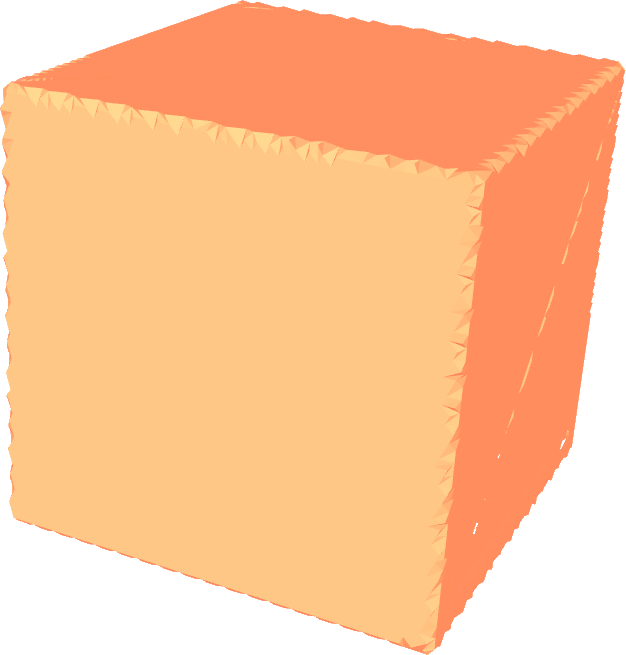
\includegraphics[width=.3\columnwidth]{figures/comparison/cube.png}
    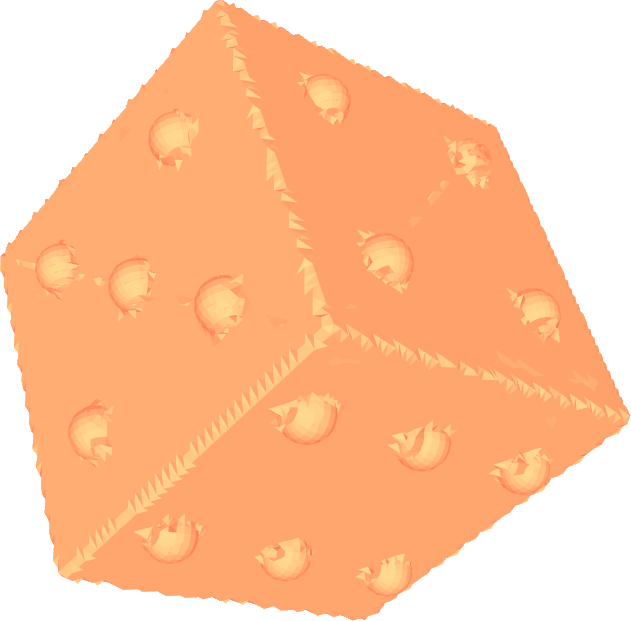
\includegraphics[width=.32\columnwidth]{figures/comparison/dice1.png}
    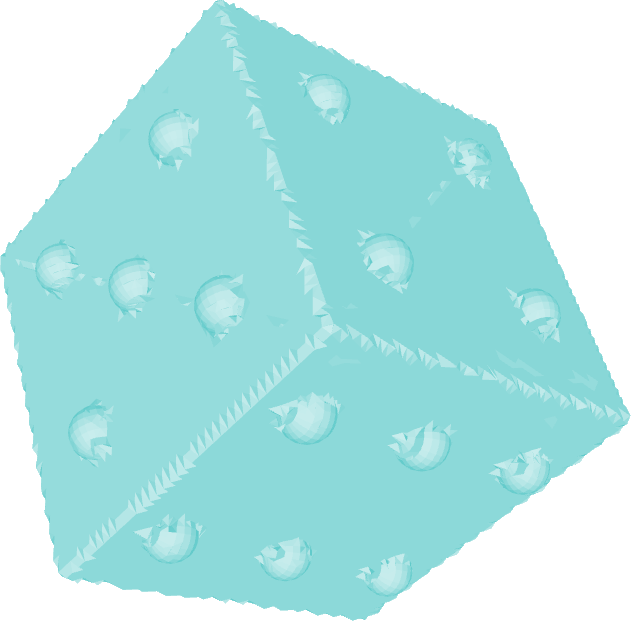
\includegraphics[width=.32\columnwidth]{figures/comparison/dice2.png}
    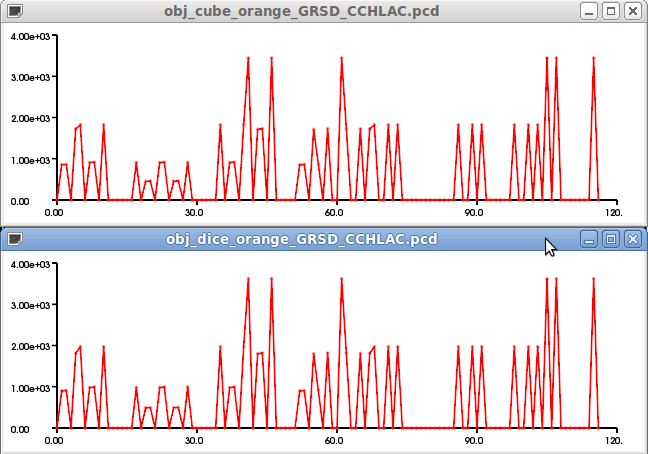
\includegraphics[width=.47\columnwidth]{figures/comparison/orange_cube_vs_orange_dice.png}
    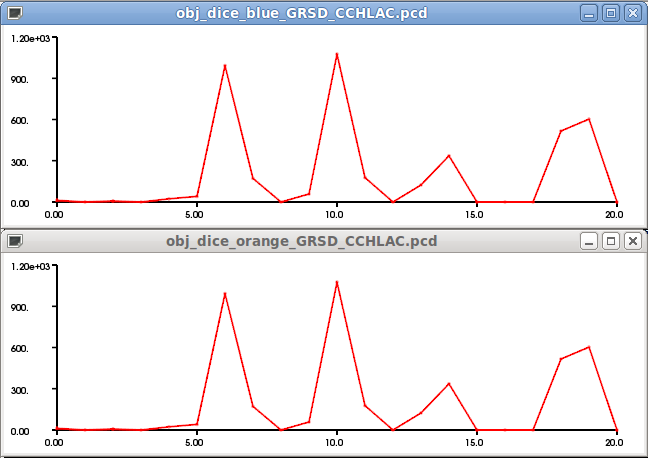
\includegraphics[width=.47\columnwidth]{figures/comparison/blue_vs_orange_dice_grsd.png}
  \caption{ColorCHLAC can not differentiate the dice from the cube (identical histograms on the left), 
    while GRSD can not differentiate the different colors (identical histograms on the right). 
    Their combination however produces different signatures for all of them (Figure~\ref{fig:grsd_cchlac}).}
  \label{fig:comparison}
\end{center}
\end{figure}

\section{Classification Methods}
\label{sec:classification}

\subsection{Linear Subspace Method}
\label{sec:subspace}
Linear Subspace Method (LSM)~\cite{watanabe1973} is an established learning method for classification. 
As a training process, several feature vectors that represent each object are extracted, 
and then Principal Component Analisis (PCA) for them is solved. 
Similarly to ~\cite{kanezaki2010icra}, we divide the whole voxel grid of each object into 
cubic subdivisions of a certain size ($7cm\times7cm\times7cm$ in our case), and then extract feature vectors from all the subdivisions for training. 
Let number of the subdivisions be $N$, the dimension of the feature vector be $d$, 
and the training feature vectors be $\bm{z}_t \in R^d, t=1,2,...N$. 
Then the eigenvectors of $R=\frac{1}{N} \sum^{N}_{t=1} \bm{z}_t \bm{z}_t^T$ are computed. 
Note that we solve PCA for all the descriptors extracted from all the trained objects for the first step, 
and the use top $d$ dimensions of the descriptor as a feature vector, in the same way as \cite{kanezaki2010icra}.

To classify and identify a detected object in environments, the system extracts one feature vector from the whole voxel grid of the object. 
Letting the feature vector be $\bm{z}$ and the matrix of top $t$ eigen vectors for the $i$-th object in the database be $P_i \equiv (\bm{v}_{i1} \bm{v}_{i2} ... \bm{v}_{ir})$,
the similarity between the query part and the $i$-th object in the database is calculated by the following equation:
\begin{eqnarray}\label{eq:y_calc}
  %\hspace{-1mm}
  y_i = \frac{\| P_i^T \bm{z} \|}{\| \bm{z} \|}
\end{eqnarray}
There is an advantage of using LSM with this kind of histogram-based descriptors which have additive property. 
The additive property means that a global descriptor for an object cluster equals the summation of local descriptors of its sub-parts. 
Owing to the property, one feature vector computed from each object cluster in environments can be classified by projecting it to 
each subspace of database object, regardless of the size of the object cluster, thus providing a method for classifying partially visible objects.

\subsection{Support Vector Machine-based Classification}
We also performed classification using Support Vector Machines (SVM)~\cite{svm99} in our experiments.
SVM is a fast classification method that works by learning the vectors that define hyperplanes separating
the training examples according to a cost and a kernel function.

Unlike LSM, it is not well suited for recognizing partially visible objects using the presented features,
unless partial views are explicitly trained. Another problem is overfitting to the training data, which
can be limited by choosing the parameters such that they maximize the results of cross-validation checks
on the training data.

We used a C-SVC type SVM with a radial basis function kernel \cite{LIBSVM}
\todo{I will put in the optimal parameters as soon as we decide on one}
\todo{we should mention scaling we used for both methods, and that example histograms are not always scaled...}

\section{Results}
\label{sec:results}
To evaluate the proposed features we ran
tests using SVM and LSM classifiers on the following two sets of data: 
i)~7 artificially generated objects with 7 different colors, and
ii)~63 objects of daily use, scanned using a Kinect sensor and a rotating table
(shown in bottom part of Figure~\ref{fig:robot}). 
We measured the recognition rates against the original implementations of ColorCHLAC and 
GRSD. Since ColorCHLAC was already shown to outperform Textured Spin Images
we did not include it in our experiments.

\subsection{Feature Extraction}
\label{sec:feature_extraction}
In all tests we parametrized the computation of the feature with the following parameters:
\begin{itemize}
\item search radius for normals: $2cm$
\item search radius for $r_{min}$ and $r_{max}$ estimation: $1cm$
\item voxel size: $1cm$
\end{itemize}

The execution times for VOSCH feature estimation are shown in the following table, where 
$\overline{nr_{points}}$ denotes the average number of points per object,
$t_{point}$ is the average estimation time per point,
and $t_{object}$ is the average estimation time needed for an object:
\newcommand{\mc}[3]{\multicolumn{#1}{#2}{#3}}
\definecolor{tcA}{rgb}{0.784314,0.784314,0.784314}
\begin{table}[ht]
\begin{center}
\begin{tabular}{|c|c|c|c|}
\hline
\rowcolor{tcA} & $\overline{nr_{points}}$ & $t_{point}$ & $t_{object}$ \\
\hline
\mc{1}{|>{\columncolor{tcA}}c|}{synthetic data (49 views of 49 objects)} & 19124 & 36$\mu s$ & 0.69s \\
\hline
\mc{1}{|>{\columncolor{tcA}}c|}{real data (1512 views of 63 objects)} & 4632 & 57$\mu s$ & 0.26s \\
\hline
\end{tabular}
\caption{Time needed for the estimation of VOSCH features.}
\label{tbl:timing}
\end{center}
\end{table}

\subsection{Synthetic Data}
We first carried out tests on a set of 49 artificially generated objects,
7 shapes, each in 7 colors (Figure~\ref{fig:grsd_cchlac}). We used 1 example of 
each object as a training sample and evaluated the model on 5 examples of each object with 
10 different noise levels. The noise levels were generated for points' 3D coordinates 
using Gaussian distribution with the following standard deviations:\\
\begin{center}
$\sigma = \{0.5, 1.0, 1.5, 2.0, 2.5, 3.0, 3.5, 4.0, 4.5, 5.0\}mm$ 
\end{center}
For LSM classification we set the dimension of the compressed feature space $d$ as 50 for ColorCHLAC, ConVOSCH and VOSCH, while 
we used full 20 dimensions of GRSD. The dimensionality of the subspace $t$ was set to 3.
The results of the test are presented in Table~\ref{tbl:synthetic},
showing VOSCH (right-most two columns) outperforming all other features.
For a better overview of the results using VOSCH please see Figure~\ref{fig:plot}

\begin{figure}[htb!]
  \begin{center}
    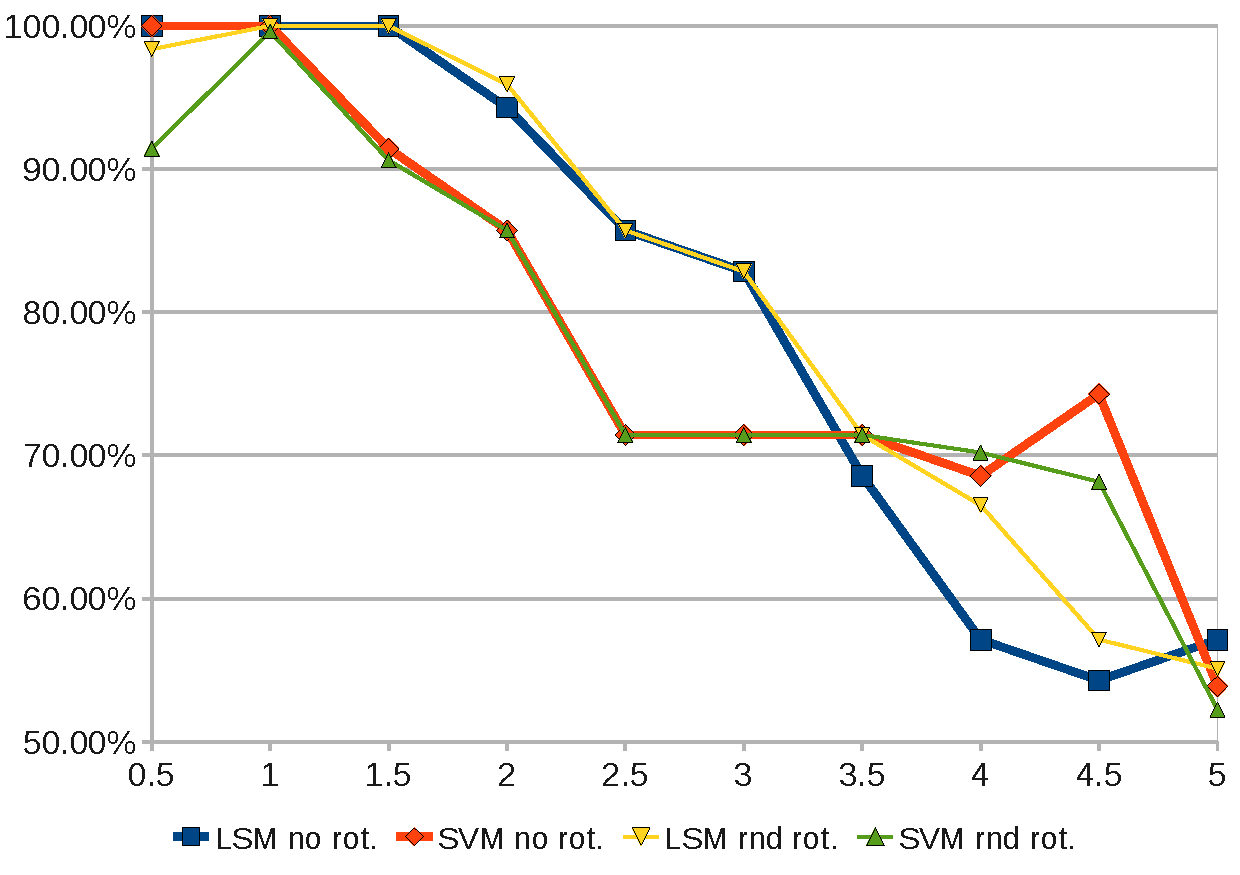
\includegraphics[width=.98\columnwidth]{figures/comparison/vosch.pdf}
    \caption{The effect of simulated noise on the classification results using VOSCH with LSM and SVM
             (both with and without random rotations of test data, as presented in Table~\ref{tbl:synthetic}).}
    \label{fig:plot}
  \end{center}
\end{figure}

Since GRSD is insensitive to color, it can identify at most $1/7 \approx 14.2857\%$ of the data.
Additionally, since objects were uniformly colored and symmetrical, the fact that ColorCHLAC 
is not rotation invariant did not expose in the table. In the original implementation ColorCHLAC 
had to be trained with the artificial rotations to achieve rotation invariance.

\begin{table*}[ht!]
\begin{center}
\begin{tabular}{|c|c|c|c|c|c|c|c|c|c|}\hline
% use packages: color,colortbl
\rowcolor{tcA} \textbf{} & \textbf{} & \mc{2}{>{\columncolor{tcA}}c|}{\textbf{GRSD/20D}} & \mc{2}{>{\columncolor{tcA}}c|}{\textbf{ColorCHLAC/981D}} & \mc{2}{>{\columncolor{tcA}}c|}{\textbf{ConVOSCH/1001D}} & \mc{2}{>{\columncolor{tcA}}c|}{\textbf{VOSCH/137D}}\\
\cline{3-10}
\rowcolor{tcA} \textbf{Noise STD} & \textbf{Rotation} & \textbf{LSM} & \textbf{SVM} & \textbf{LSM} & \textbf{SVM} & \textbf{LSM} & \textbf{SVM} & \textbf{LSM} & \textbf{SVM}\\
\hline
\mc{1}{|>{\columncolor{tcA}}c|}{\textbf{0.5}} & \mc{1}{>{\columncolor{tcA}}c|}{\textbf{None:}} & 14.2857\% & 14.2857\% & 100\% & 100\% & 85.7142\% & 100\% & 100\% & 100\% \\
\rowcolor{tcA} \textbf{mm} & \textbf{Random:} & 14.2857\% & 12.6531\% & 35.1020\% & 70.2041\% & 83.2653\% & 79.5918\% & 98.3673\% & 91.4286\% \\
\hline
\mc{1}{|>{\columncolor{tcA}}c|}{\textbf{1.0}} & \mc{1}{>{\columncolor{tcA}}c|}{\textbf{None:}} & 14.2857\% & 14.2857\% & 71.4285\% & 77.1429\% & 85.7142\% & 85.7143\% & 100\% & 100\% \\
\rowcolor{tcA} \textbf{mm} & \textbf{Random:} & 14.2857\% & 14.2857\% & 34.6938\% & 65.7143\% & 82.8571\% & 78.7755\% & 100\% & 99.5918\% \\
\hline
\mc{1}{|>{\columncolor{tcA}}c|}{\textbf{1.5}} & \mc{1}{>{\columncolor{tcA}}c|}{\textbf{None:}} & 14.2857\% & 13.0612\% & 54.2857\% & 28.5714\% & 85.7142\% & 85.7143\% & 100\% & 91.4286\% \\
\rowcolor{tcA} \textbf{mm} & \textbf{Random:} & 14.2857\% & 13.0612\% & 20.4081\% & 26.1224\% & 81.6326\% & 82.449\% & 100\% & 90.6122\% \\
\hline
\mc{1}{|>{\columncolor{tcA}}c|}{\textbf{2.0}} & \mc{1}{>{\columncolor{tcA}}c|}{\textbf{None:}} & 13.8775\% & 12.2449\% & 28.5714\% & 28.5714\% & 73.4693\% & 85.7143\% & 94.2857\% & 85.7143\% \\
\rowcolor{tcA} \textbf{mm} & \textbf{Random:} & 13.4693\% & 12.2449\% & 17.1428\% & 20.8163\% & 67.3469\% & 85.7143\% & 95.9183\% & 85.7143\% \\
\hline
\mc{1}{|>{\columncolor{tcA}}c|}{\textbf{2.5}} & \mc{1}{>{\columncolor{tcA}}c|}{\textbf{None:}} & 12.2448\% & 10.2041\% & 28.5714\% & 28.5714\% & 57.9591\% & 57.1429\% & 85.7142\% & 71.4286\% \\
\rowcolor{tcA} \textbf{mm} & \textbf{Random:} & 12.2448\% & 10.2041\% & 16.3265\% & 25.7143\% & 51.4285\% & 57.1429\% & 85.7142\% & 71.4286\% \\
\hline
\mc{1}{|>{\columncolor{tcA}}c|}{\textbf{3.0}} & \mc{1}{>{\columncolor{tcA}}c|}{\textbf{None:}} & 12.2448\% & 10.2041\% & 28.5714\% & 28.5714\% & 57.1428\% & 57.1429\% & 82.8571\% & 71.4286\% \\
\rowcolor{tcA} \textbf{mm} & \textbf{Random:} & 12.2448\% & 10.2041\% & 17.5510\% & 28.5714\% & 53.8775\% & 55.5102\% & 82.8571\% & 71.4286\% \\
\hline
\mc{1}{|>{\columncolor{tcA}}c|}{\textbf{3.5}} & \mc{1}{>{\columncolor{tcA}}c|}{\textbf{None:}} & 11.0204\% & 10.2041\% & 28.5714\% & 28.5714\% & 57.1428\% & 57.1429\% & 68.5714\% & 71.4286\% \\
\rowcolor{tcA} \textbf{mm} & \textbf{Random:} & 11.8367\% & 10.2041\% & 15.5102\% & 28.5714\% & 50.2040\% & 45.3061\% & 71.4285\% & 71.4286\% \\
\hline
\mc{1}{|>{\columncolor{tcA}}c|}{\textbf{4.0}} & \mc{1}{>{\columncolor{tcA}}c|}{\textbf{None:}} & 8.9795\% & 8.57143\% & 25.7142\% & 28.5714\% & 49.7959\% & 43.2653\% & 57.1428\% & 68.5714\% \\
\rowcolor{tcA} \textbf{mm} & \textbf{Random} &  9.7959\% & 8.57143\% & 15.1020\% & 28.5714\% & 39.5918\% & 42.8571\% & 66.5306\% & 70.2041\% \\
\hline
\mc{1}{|>{\columncolor{tcA}}c|}{\textbf{4.5}} & \mc{1}{>{\columncolor{tcA}}c|}{\textbf{None:}} & 7.3469\% & 8.16327\% & 14.2857\% & 28.5714\% & 42.8571\% & 42.8571\% & 54.2857\% & 74.2857\% \\
\rowcolor{tcA} \textbf{mm} & \textbf{Random:} & 7.7551\% & 7.7551\% & 15.1020\% & 28.5714\% & 34.2857\% & 44.898\% & 57.1428\% & 68.1633\% \\
\hline
\mc{1}{|>{\columncolor{tcA}}c|}{\textbf{5.0}} & \mc{1}{>{\columncolor{tcA}}c|}{\textbf{None:}} & 8.1632\% & 5.71429\% & 14.2857\% & 28.5714\% & 42.4489\% & 53.4694\% & 57.1428\% & 53.8776\% \\
\rowcolor{tcA} \textbf{mm} & \textbf{Random:} & 8.5714\% & 6.12245\% & 15.5102\% & 28.5714\% & 32.6530\% & 52.6531\% & 55.1020\% & 52.2449\% \\
\hline
\end{tabular}
\caption{Comparison of the features and classifiers using both test data in the same pose as the training data, and randomly rotated test data.}
\label{tbl:synthetic}
\end{center}
\end{table*}


\subsection{Real Data}
\subsubsection{Acquisition of Training Data}
Our database of 3D objects was obtained using the Kinect sensor.
The set of objects (see Figure~\ref{fig:robot}) encompasses the ones commonly used
in a typical household environment (mugs, utensils, groceries, etc) and is envisioned for a
larger expansion and release after the review process.  We rotated the objects on the rotating table with
an angular step of $15^\circ$, and acquired partial
snapshots using the same sensor and from a perspective that best
approximates the robot's view point during its working cycle.  We consider
this to be an important point as opposed to similar initiatives (e.g.,
\cite{kit}) where the datasets are acquired using high-precision fixed sensors.

% \begin{figure}[htb!]
%   \begin{center}
%     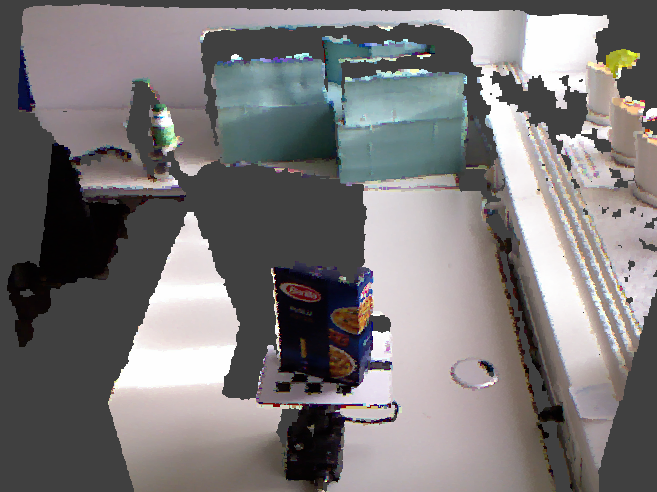
\includegraphics[width=.32\columnwidth]{figures/rot_table/barilla.png}
%     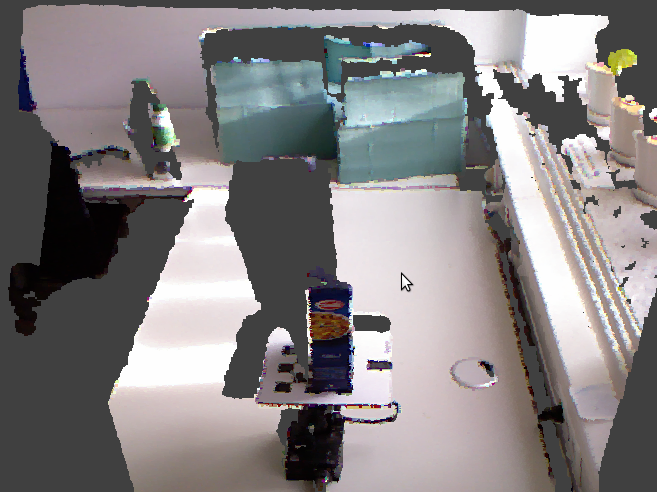
\includegraphics[width=.32\columnwidth]{figures/rot_table/barilla1.png}
%     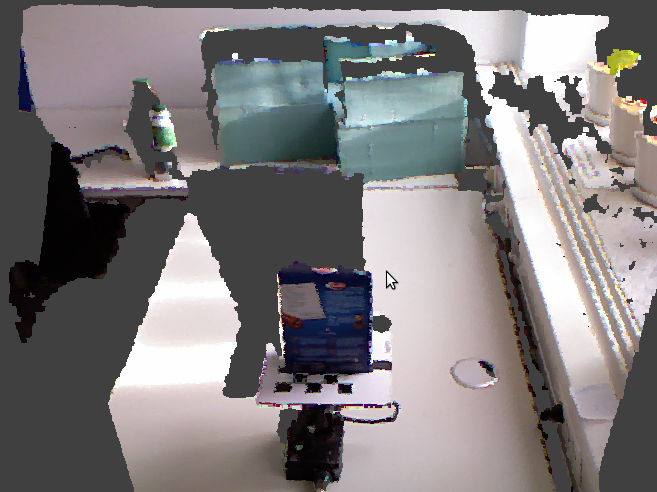
\includegraphics[width=.32\columnwidth]{figures/rot_table/barilla2.png}
%     \caption{Acquisition of training data using a rotating table controlled by the robot.}
%     \label{fig:data_acquisition}
%   \end{center}
% \end{figure}

\begin{figure}[htb!]
  \begin{center}
    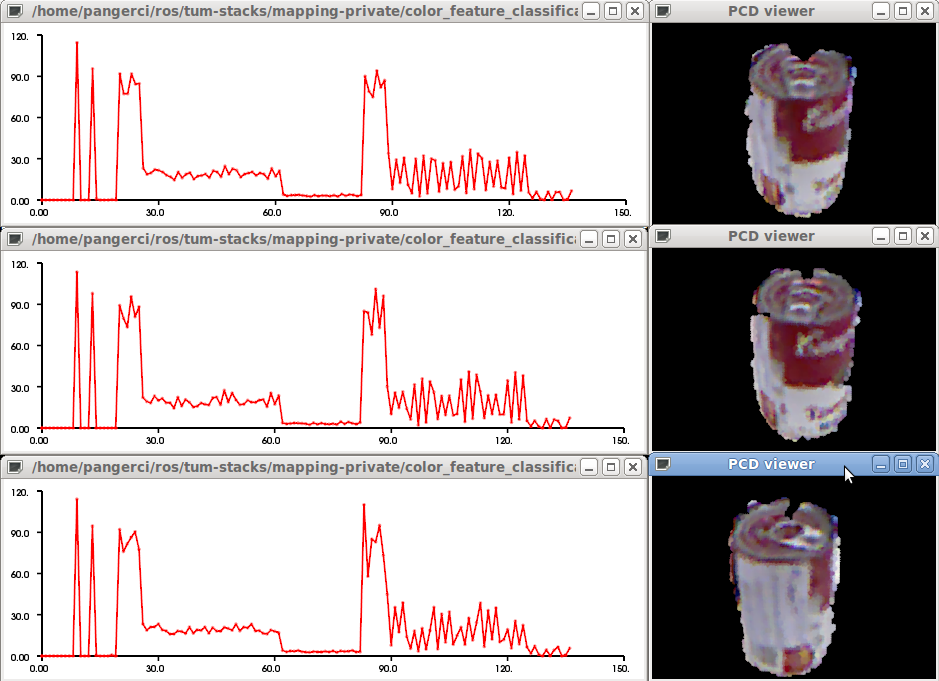
\includegraphics[width=.9\columnwidth]{figures/colorCHLAC/real/tomato/tomato_hist_pcd.png}
    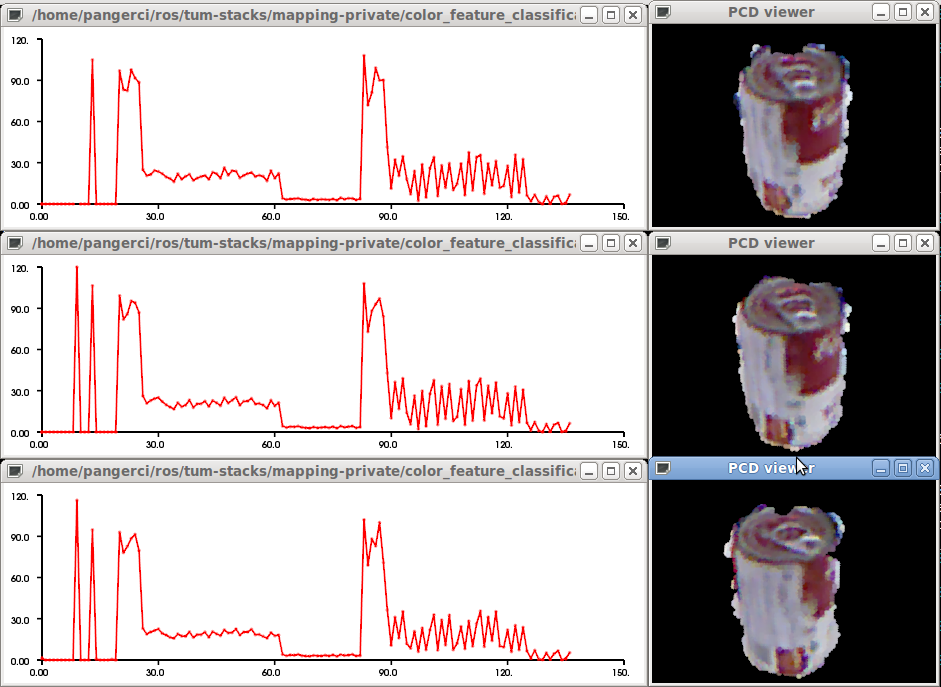
\includegraphics[width=.9\columnwidth]{figures/colorCHLAC/real/tomato/tomato_hist_pcd2.png}
    \caption{Examples of \todo{scaled} VOSCH histograms for a tomato soup can.}
    \label{fig:grsd_colorchlac_tomato}
  \end{center}
\end{figure}


\subsubsection{Evaluation on Training Data}
Table~\ref{tbl:training} shows the percentage of correctly classified training examples using the model computed for them.
The numbers in parentheses are the percentages of correctly classified views using the model constructed using the remaining views
(leave-one-out-test).

% \begin{table*}[ht]
% \begin{center}
% \begin{tabular}{|c|c|c|c|c|}
% \hline
% \rowcolor{tcA} & \textbf{GRSD (20D)} & \textbf{Color-CHLAC (981D)} & \textbf{Concatenated (ConVOSCH)} & \textbf{VOSCH (137D)} \\
% \hline
% \mc{1}{|>{\columncolor{tcA}}c|}{\textbf{LSM}} & 29.6958\% (17.2619\%) & 99.0741\% (97.8175\%) & 99.3386\% (96.8915\%) & 97.8836\% (93.1217\%) \\
% \hline
% \mc{1}{|>{\columncolor{tcA}}c|}{\textbf{SVM}} & 99.2063\% (66.9974\%) & 99.8677\% (99.6693\%)  & 99.9339\% (99.6032\%) & 100\% (99.1402\%) \\
% \hline
% \end{tabular}
% \caption{Model Accuracy on Training Data (and Leave-One-Out Test) for VOSCH \todo{less decimals and 1 column}}
% \label{tbl:training}
% \end{center}
% \end{table*}

\begin{table}[ht]
\begin{footnotesize}
\begin{center}
\begin{tabular}{|c|c|c|c|c|}
\hline
\rowcolor{tcA} & \textbf{GRSD} & \textbf{ColorCHLAC} & \textbf{ConVOSCH} & \textbf{VOSCH} \\
\rowcolor{tcA} & \textbf{20D [\%]} & \textbf{981D [\%]} & \textbf{1001D [\%]} & \textbf{137D [\%]} \\
\hline
\mc{1}{|>{\columncolor{tcA}}c|}{\textbf{LSM}} & 29.7 (17.26) & 99.07 (97.82) & 99.34 (96.89) & 97.88 (93.12) \\
\hline
\mc{1}{|>{\columncolor{tcA}}c|}{\textbf{SVM}} & 99.21 (67) & 99.87 (99.67)  & 99.93 (99.6) & 100 (99.14) \\
\hline
\end{tabular}
\caption{Model Accuracy on Training Data and Leave-One-Out Test}
\label{tbl:training}
\end{center}
\end{footnotesize}
\end{table}

\subsubsection{Evaluation on Novel Views}
To evaluate the proposed features on novel views as well, we performed the test with the
following setup (shown in Figure~\ref{fig:novel_views}): we selected 4 types of scenes containing textured
and textureless objects (a and b), objects with similar shapes (c) and a scene with the substantial 
altered lighting conditions (d). We acquired the data from 3 substantially different views 
as shown in Figure~\ref{fig:novel_views}, and object candidate clusters were detected
by first finding a major horizontal planar surface within the point cloud, as done in~\cite{Rusu09IROS_ClosingLoop}.
For these experiments we set 15 as the dimension of subspace $t$ in LSM. 

\begin{table}[ht]
\begin{scriptsize}
\begin{center}
\begin{tabular}{|c|c|c|c|c|c|}
\hline
\rowcolor{tcA} & \textbf{} & \textbf{GRSD} & \textbf{ColorCHLAC} & \textbf{ConVOSCH} & \textbf{VOSCH} \\
\rowcolor{tcA} & \textbf{} & \textbf{20D} & \textbf{981D} & \textbf{1001D} & \textbf{137D} \\
\hline
\mc{1}{|>{\columncolor{tcA}}c|}{\textbf{(a)}} & \mc{1}{>{\columncolor{tcA}}c|}{\textbf{LSM}} & 16.7\% & 58.3\% & 75\% & 75\% \\
\mc{1}{|>{\columncolor{tcA}}c|}{\textbf{texture}} & \mc{1}{>{\columncolor{tcA}}c|}{{SVM}} & 33.3\% & 66.7\% & 75\% & 66.7\% \\
\hline
\mc{1}{|>{\columncolor{tcA}}c|}{\textbf{(b)}} & \mc{1}{>{\columncolor{tcA}}c|}{\textbf{LSM}} & 11.1\% & 33.3\% & 38.9\% & 44.4\% \\
\mc{1}{|>{\columncolor{tcA}}c|}{\textbf{no texture}} & \mc{1}{>{\columncolor{tcA}}c|}{{SVM}} & 27.8\% & 61.1\% & 61.1\% & 50\% \\
\hline
\mc{1}{|>{\columncolor{tcA}}c|}{\textbf{(c)}} & \mc{1}{>{\columncolor{tcA}}c|}{\textbf{LSM}} & 5.56\% & 33.3\% & 44.4\% & 61.1\% \\
\mc{1}{|>{\columncolor{tcA}}c|}{\textbf{sim. shape}} & \mc{1}{>{\columncolor{tcA}}c|}{\textbf{SVM}} & 27.8\% & 77.8\% & 77.8\% & 77.8\% \\
\hline
\mc{1}{|>{\columncolor{tcA}}c|}{\textbf{(d)}} & \mc{1}{>{\columncolor{tcA}}c|}{\textbf{LSM}} & 5.56\% & 50\% & 72.2\% & 55.6\% \\
\mc{1}{|>{\columncolor{tcA}}c|}{\textbf{diff. light}} & \mc{1}{>{\columncolor{tcA}}c|}{\textbf{SVM}} & 11.1\% & 88.9\% & 88.9\% & 83.3\% \\
\hline
\mc{1}{|>{\columncolor{tcA}}c|}{\textbf{(e)}} & \mc{1}{>{\columncolor{tcA}}c|}{\textbf{LSM}} &  &  &  &  \\
\mc{1}{|>{\columncolor{tcA}}c|}{\textbf{...}} & \mc{1}{>{\columncolor{tcA}}c|}{\textbf{SVM}} &  &  &  &  \\
\hline
\hline
\mc{1}{|>{\columncolor{tcA}}c|}{\textbf{Average}} & \mc{1}{>{\columncolor{tcA}}c|}{\textbf{LSM}} &  &  &  &  \\
\mc{1}{|>{\columncolor{tcA}}c|}{\textbf{and STD}} & \mc{1}{>{\columncolor{tcA}}c|}{\textbf{SVM}} &  &  &  &  \\
\hline
\end{tabular}
\end{center}
\end{scriptsize}
\caption{Model accuracy on novel view data.}
\label{tbl:novel}
\end{table}

%% \todo{Prove it works for a)textured objects, b)texture-less objects, c)objects with different shapes, 
%% d)varying lighting conditions -- no clutter, 1 object at a time}
%\todo{Dejan}

\subsection{Object Detection Pipeline (in Clutter)}
\label{sec:recognition}
We applied our object recognition method on an object detection scheme in a cluttered environment.
The system computes the similarities between each target object and all rectangular-solid sub-regions in the environment, and then it outputs all the regions that have higher similarities than a certain threshold as the candidates of the target object.
Each sub-region has the same size as that of the bounding box of the target object.
To accelerate feature extraction from the sub-regions, we used ``Integral Feature Table''~\cite{kanezaki2010tvc}, which is a simple extension of ``Integral Image''~\cite{viola2001} from 2D to 3D.
The ``Integral Feature Table'' $\bm{I}(x,y,z)$ is defined as the $d$-dimensional compressed feature vector extracted from the voxel area
    ranging from $(0,0,0)$ to $(x,y,z)$.
Let the feature vector of the voxel area with $x$ ranging from $x_1$ to $x_2$,
    $y$ ranging from $y_1$ to $y_2$, and $z$ ranging from $z_1$ to $z_2$, be $\bm{F}(x_1,y_1,z_1,x_2,y_2,z_2)$.
This is computed by the following equation:
\begin{eqnarray*}\label{eq:sat}
\bm{F}(x_1,y_1,z_1,x_2,y_2,z_2) = \bm{I}(x_2,y_2,z_2) - \bm{I}(x_1,y_2,z_2)
                           \\ - \bm{I}(x_2,y_1,z_2) - \bm{I}(x_2,y_2,z_1)
                           \\ + \bm{I}(x_1,y_1,z_2) + \bm{I}(x_1,y_2,z_1)
                           \\ + \bm{I}(x_2,y_1,z_1) - \bm{I}(x_1,y_1,z_1)
\end{eqnarray*}
Using the ``Integral Feature Table'', $\bm{F}(x_1,y_1,z_1,x_2,y_2,z_2)$ can always be computed by adding the 8 cached feature vectors,
    regardless of the size of the target object.
Note that this is not effective when the number of sub-regions included in the detection box is smaller than 8.
Within the large color voxel data of an environment,
   only the voxels on the surface of each object have RGB values, while other voxels have the empty property.
This means that the object detection process can be accelerated by skipping empty regions.
Similarly to the ``Integral Feature Table'', we create a table that stores
   the number of voxels with the occupied property, in the area ranging from $(0,0,0)$ to $(x,y,z)$.
Using this table, the number of voxels with the occupied property in the detection box can be computed quickly by adding 8 scalar values.
If the number is less than a certain threshold $h$,
   the system skips the similarity calculation and moves the detection box forwards.
In this work, we set $h$ to the minimum value of the occupied voxel number in the training samples of the target object.

\todo{Asako: description for the results}

\begin{figure*}[htb!]
  \centering
  \subfloat[Textured objects (View 1)]{\label{fig:textured}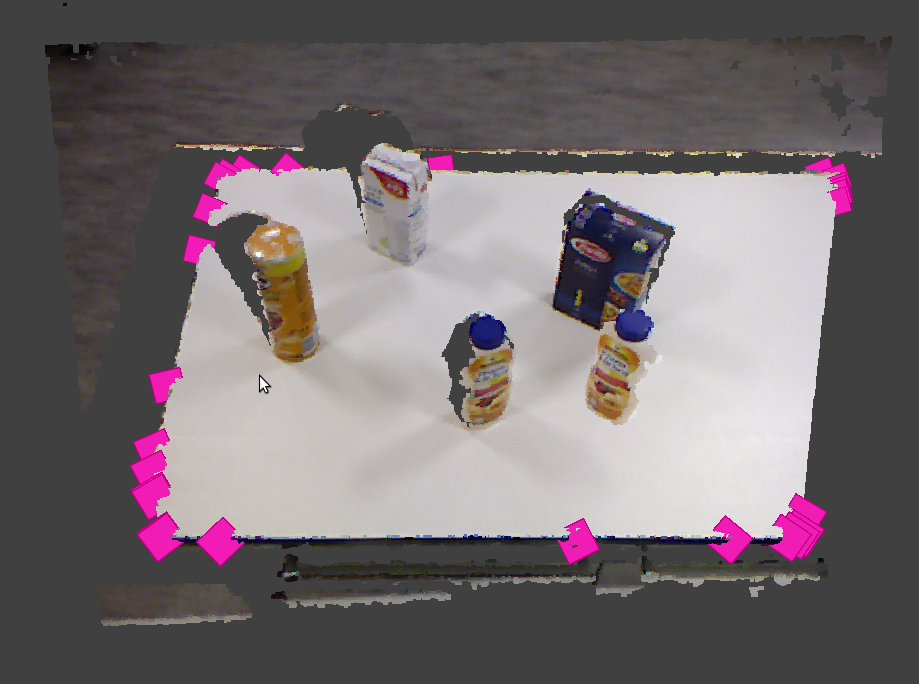
\includegraphics[width=.25\textwidth]{figures/novel_view_scenes/text_view1.png}}
  \subfloat[Textureless objects (View 2)]{\label{fig:textureless}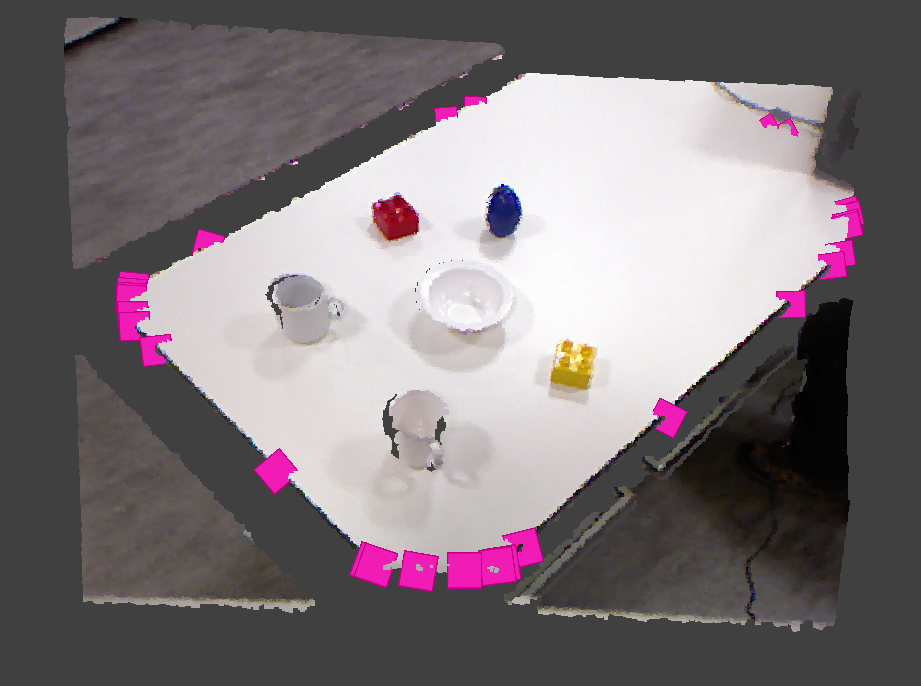
\includegraphics[width=.25\textwidth]{figures/novel_view_scenes/textureless_view2.png}}
  \subfloat[Two categories of objects with similar shapes (View 1)]{\label{fig:similar_shapes}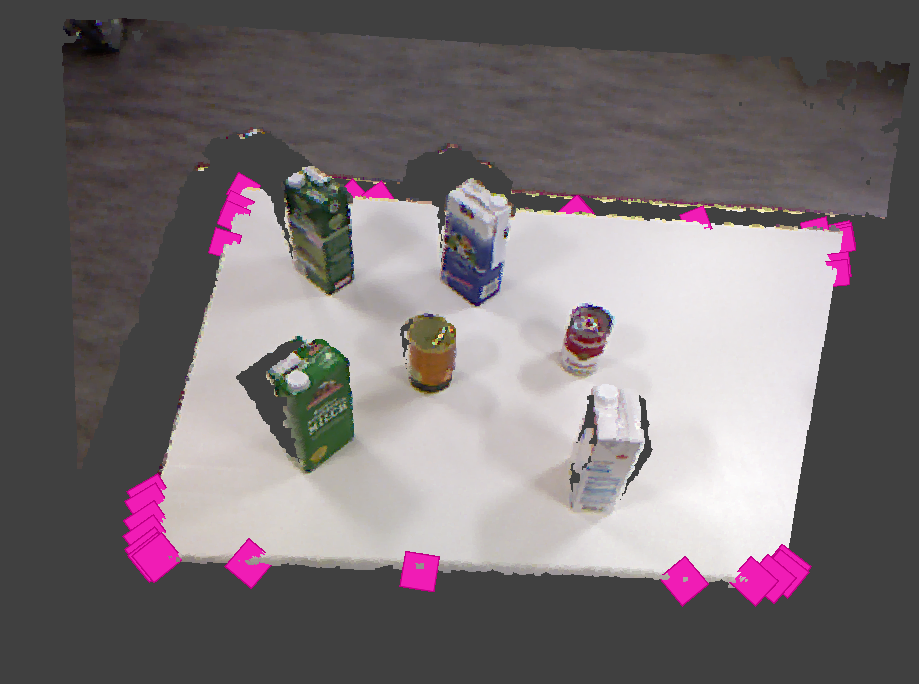
\includegraphics[width=.25\textwidth]{figures/novel_view_scenes/similar_shape_view1.png}}
  \subfloat[Altered light conditions (View 3)]{\label{fig:light}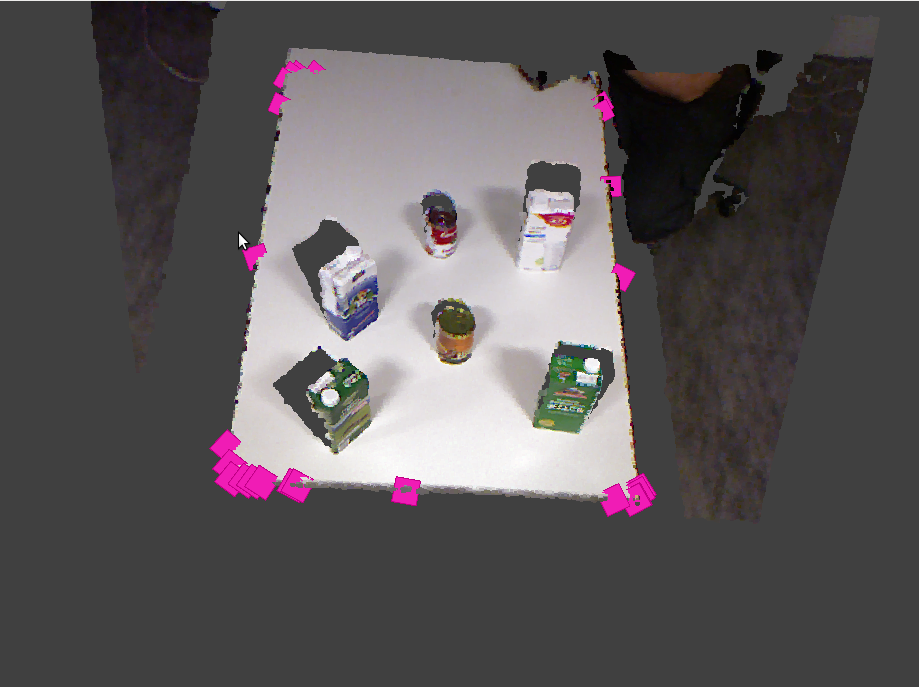
\includegraphics[width=.25\textwidth]{figures/novel_view_scenes/diff_light_view3.png}}
 \caption{Screenshots of the novel view scenes (best viewed in color)}
 \label{fig:novel_views}
\end{figure*}

\section{Conclusions and Future Work}
\label{sec:conclusion}

We presented and evaluated a way to efficiently combine two
appearance characteristics into a single feature (both rotation
variant and rotation invariant) and shown its advantage over
the original methods.

The rotation invariant VOSCH feature with its low number of dimensions
promises to be an efficient and descriptive feature that scales well with
the increased number of objects a real-world application of the system would
require. ColorCHLAC is not rotation invariant, so it has to be trained with
all rotations around the view-ray, thus ConVOSCH as well. We found
however, that at least for our 63 objects, the texture variations
were not significantly different when the objects were rotated
-- neither for the single colored synthetic data (Table~\ref{tbl:synthetic}),
nor for the real views (Table~\ref{tbl:novel}).
Since the features were designed to be additive, they can be used using
LSM and detection in cluttered scenes using a sliding box approach.

Unfortunately, acquiring enough labeled training data with enough variation
to avoid overfitting is a problem in 3D perception, thus the final results are
not completely informative and have high variations.
We try to address these issues by expanding and publishing our database of objects
and creating more labeled scenes for evaluation.
Also, the automatic building of object databases by in-hand modeling by the
robot itself is a useful tool that we plan to investigate in order to expand
our database with novel objects.
% requires grasping without recognition - cite IROS10... maybe for the final version

Future work will include incorporation of other promising 2.5/3D approaches like VFH and NARF
into the voxelized feature extraction process, and evaluating using more test and training data.

\todo{color stabilization?}


% \section*{Acknowledgments}
% This work was supported by the DFG cluster of excellence \emph{CoTeSys} (Cognition for Technical Systems). \todo{Willow?}\\
% \todo{Asako: Do we need to ackknowledge someone from ISI Lab?}
% %% Use plainnat to work nicely with natbib.

\bibliographystyle{plainnat}
\bibliography{references}
\end{document}


%TODO:
%Check the original template and see what the meant with the hyperlinks
